\documentclass[tikz,border=3mm]{standalone}
\usepackage{tikz}
\usepackage{amsmath,amssymb}
\usetikzlibrary{arrows.meta, positioning, fit, backgrounds}

\begin{document}
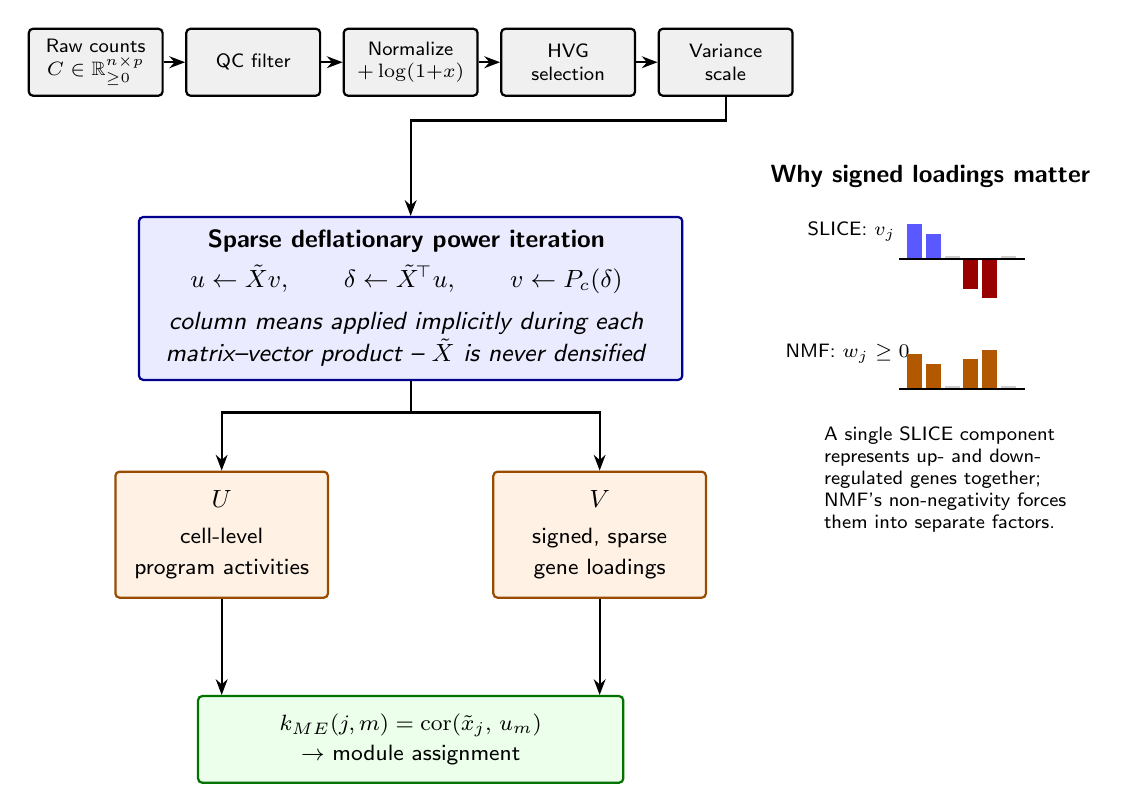
\begin{tikzpicture}[
    font=\sffamily\small,
    box/.style={draw, rounded corners=1.5pt, minimum height=0.85cm, align=center, thick},
    prep/.style={box, fill=gray!12, minimum width=1.7cm, font=\sffamily\scriptsize},
    core/.style={box, fill=blue!8, minimum width=6.9cm, minimum height=1.9cm, thick, draw=blue!55!black},
    outbox/.style={box, fill=orange!10, minimum width=2.7cm, draw=orange!60!black, minimum height=1.6cm},
    kmebox/.style={box, fill=green!8, minimum width=5.4cm, minimum height=1.1cm, draw=green!45!black},
    arr/.style={-{Stealth[length=2mm]}, thick},
]

% ============ main pipeline (unchanged from validated version) ============
\node[prep] (raw)   at (0.0, 8) {Raw counts\\ $C \in \mathbb{R}_{\ge 0}^{n\times p}$};
\node[prep] (qc)    at (2.0, 8) {QC filter};
\node[prep] (norm)  at (4.0, 8) {Normalize\\ $+\log(1{+}x)$};
\node[prep] (hvg)   at (6.0, 8) {HVG\\ selection};
\node[prep] (scale) at (8.0, 8) {Variance\\ scale};
\draw[arr] (raw) -- (qc);
\draw[arr] (qc) -- (norm);
\draw[arr] (norm) -- (hvg);
\draw[arr] (hvg) -- (scale);

\node[core] (core) at (4.0, 5) {
  \begin{tabular}{c}
  \textbf{Sparse deflationary power iteration} \\[3pt]
  $u \leftarrow \tilde X v, \qquad \delta \leftarrow \tilde X^{\!\top} u, \qquad v \leftarrow P_c(\delta)$ \\[4pt]
  \small\textit{column means applied implicitly during each} \\
  \small\textit{matrix--vector product -- $\tilde X$ is never densified}
  \end{tabular}
};
\draw[arr] (scale.south) -- ++(0,-3mm) -| (core.north);

\node[outbox] (U) at (1.6, 2) {$U$\\[2pt] \footnotesize cell-level\\ \footnotesize program activities};
\node[outbox] (V) at (6.4, 2) {$V$\\[2pt] \footnotesize signed, sparse\\ \footnotesize gene loadings};
\draw[arr] (core.south) -- ++(0,-4mm) -| (U.north);
\draw[arr] (core.south) -- ++(0,-4mm) -| (V.north);

\node[kmebox] (kme) at (4.0, -0.6) {
  \footnotesize $k_{ME}(j,m) = \mathrm{cor}(\tilde x_j,\, u_m)$ \\
  \footnotesize $\to$ module assignment
};
\draw[arr] (U.south) -- ++(0,-5mm) -| (kme.north -| U.south);
\draw[arr] (V.south) -- ++(0,-5mm) -| (kme.north -| V.south);

% ============ side panel: why signed loadings matter (own clean column) ============
\node[box, draw=none, fill=none, font=\sffamily\bfseries\small] (panel_title) at (10.6, 6.55) {Why signed loadings matter};

\node[font=\sffamily\scriptsize] (slice_lab) at (9.6, 5.85) {SLICE: $v_j$};
\begin{scope}[xshift=10.3cm, yshift=5.5cm]
  \foreach \i/\h/\c in {0/0.45/blue!65, 1/0.32/blue!65, 2/0.04/gray!40, 3/-0.38/red!60!black, 4/-0.5/red!60!black, 5/0.04/gray!40}
    \draw[fill=\c, draw=none] (\i*0.24, 0) rectangle ++(0.19, \h);
  \draw[thick] (-0.1,0) -- (1.5,0);
\end{scope}

\node[font=\sffamily\scriptsize] (nmf_lab) at (9.55, 4.3) {NMF: $w_j \ge 0$};
\begin{scope}[xshift=10.3cm, yshift=3.85cm]
  \foreach \i/\h/\c in {0/0.45/orange!70!black, 1/0.32/orange!70!black, 2/0.04/gray!40, 3/0.38/orange!70!black, 4/0.5/orange!70!black, 5/0.04/gray!40}
    \draw[fill=\c, draw=none] (\i*0.24, 0) rectangle ++(0.19, \h);
  \draw[thick] (-0.1,0) -- (1.5,0);
\end{scope}

\node[font=\sffamily\scriptsize, text width=3.3cm, align=left] at (10.9, 2.7) {A single SLICE component represents up- and down-regulated genes together; NMF's non-negativity forces them into separate factors.};

\end{tikzpicture}
\end{document}
